\documentclass[12pt,a4paper]{article}
\usepackage[utf8]{inputenc}
\usepackage[vietnamese]{babel}
\usepackage{graphicx}
\usepackage{float}
\usepackage{geometry}
\geometry{a4paper, margin=2.5cm}
\usepackage{hyperref}
\usepackage{xcolor}
\usepackage{fancyhdr}
\usepackage{titlesec}
\usepackage{booktabs}
\usepackage{array}

\hypersetup{
    colorlinks=true,
    linkcolor=blue,
    filecolor=magenta,      
    urlcolor=cyan,
    pdftitle={Bao cao Bai tap 5 - AI tao sinh trong sang tao noi dung},
    pdfpagemode=FullScreen,
}

% Cấu hình header & footer
\pagestyle{fancy}
\fancyhf{}
\rhead{Hành trình Kỹ năng số}
\lhead{Bài tập Thực hành 5}
\rfoot{Trang \thepage}

% Định dạng tiêu đề mục
\titleformat{\section}{\normalfont\Large\bfseries\color{blue!80!black}}{\thesection}{1em}{}
\titleformat{\subsection}{\normalfont\large\bfseries\color{blue!60!black}}{\thesubsection}{1em}{}

\begin{document}

% --- TRANG BÌA ---
\begin{titlepage}
    \centering
    \vspace*{1cm}
    
    {\large \bfseries TRƯỜNG ĐẠI HỌC CÔNG NGHỆ - ĐHQGHN} \\[0.2cm]
    {\large \bfseries KHOA CÔNG NGHỆ THÔNG TIN} \\[1.5cm{}]
    
    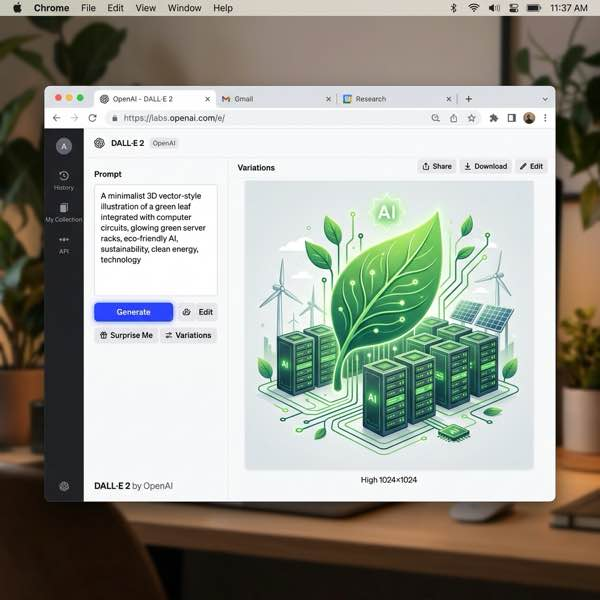
\includegraphics[width=0.3\textwidth]{images/dalle_illustration.jpg} \\[1.5cm]
    
    {\Large \bfseries BÁO CÁO BÀI TỰ THỰC HÀNH CÁ NHÂN} \\[0.5cm]
    {\Huge \bfseries BÀI TẬP 5: SÁNG TẠO NỘI DUNG SỐ VỚI AI TẠO SINH} \\[1.5cm]
    
    \textbf{Môn học:} Nhập môn Công nghệ số và Ứng dụng Trí tuệ nhân tạo \\
    \textbf{Chủ đề:} Thiết kế slide thuyết trình và Infographic về "Green AI" \\[2cm]
    
    \begin{flushleft}
        \large
        \textbf{Sinh viên thực hiện:} Nguyễn Bảo Đăng \\
        \textbf{Mã số sinh viên:} 25020115 \\
    \end{flushleft}
    
    \vfill
    {\large Năm 2026}
\end{titlepage}

\newpage
\tableofcontents
\newpage

% --- NỘI DUNG CHÍNH ---

\section{Giới thiệu Dự án và Thiết lập Công cụ}

\subsection{Ý tưởng dự án sáng tạo nội dung}
Trong bài thực hành này, tôi chọn dự án **Thiết kế slide thuyết trình (Presentation) và Infographic** giới thiệu về chủ đề \textbf{"Green AI - Trí tuệ nhân tạo xanh và phát triển bền vững"}. Đây là một chủ đề có tính thời sự cao trong ngành Khoa học Máy tính, đề cập đến việc tối ưu hóa thuật toán và phần cứng để giảm thiểu lượng điện năng tiêu thụ và lượng khí thải carbon khổng lồ sinh ra từ việc huấn luyện các mô hình AI lớn.

Sản phẩm cuối cùng của dự án gồm 2 phần:
\begin{enumerate}
    \item Bộ slide thuyết trình 5 trang cung cấp cái nhìn tổng quan về thách thức và giải pháp của Green AI.
    \item Một Infographic định dạng dọc tóm tắt các số liệu thực trạng và hành động thực tiễn.
\end{enumerate}

\subsection{Các công cụ AI tạo sinh được lựa chọn}
Để thực hiện dự án này, tôi sử dụng kết hợp 3 công cụ AI tạo sinh thuộc các nhóm tính năng khác nhau:
\begin{itemize}
    \item \textbf{ChatGPT (so sánh với Gemini)}: Nhóm AI tạo văn bản, hỗ trợ phác thảo dàn ý kịch bản slide thuyết trình và tìm kiếm ý tưởng số liệu cho Infographic.
    \item \textbf{DALL-E 2 / Midjourney}: Nhóm AI tạo hình ảnh, hỗ trợ sinh ra các bức ảnh minh họa 3D vector độc quyền về biểu tượng Green AI (chiếc lá tích hợp vi mạch và máy chủ).
    \item \textbf{Canva Magic Design}: Nhóm AI hỗ trợ thiết kế, giúp tạo bố cục slide thuyết trình ban đầu dựa trên văn bản đầu vào.
\end{itemize}

\newpage
\section{Nhật ký chi tiết quá trình sử dụng AI}
Dưới đây là nhật ký ghi nhận chi tiết các bước sử dụng AI, các prompt thực tế và so sánh kết quả thực hiện.

\subsection{Bước 1: Lên ý tưởng nội dung với ChatGPT và Gemini}
Tôi đã sử dụng một prompt chi tiết trên ChatGPT để lập đề cương cho 5 slide thuyết trình và bố cục Infographic:
\\ \texttt{"Bạn là chuyên gia về Công nghệ xanh. Hãy phác thảo cấu trúc 5 slide thuyết trình và bố cục Infographic về 'Green AI - Trí tuệ nhân tạo xanh'. Nội dung slide cần súc tích, chuyên nghiệp; Infographic cần sáng tạo, trực quan, dễ hiểu. Cảm ơn!"}

\begin{figure}[H]
    \centering
    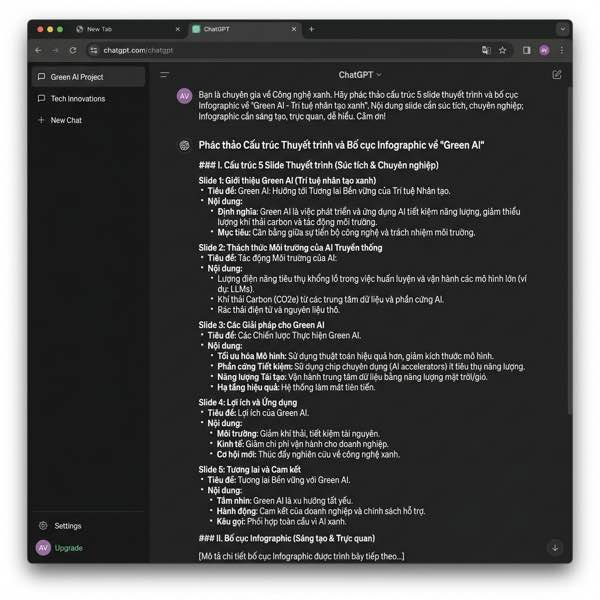
\includegraphics[width=0.85\textwidth]{images/chatgpt_script.jpg}
    \caption{ChatGPT lập cấu trúc chi tiết cho các slide thuyết trình Green AI}
    \label{fig:chatgpt_script}
\end{figure}

Để có góc nhìn khách quan, tôi thực hiện câu lệnh tương tự trên Google Gemini để tiến hành so sánh đối chiếu:
\\ \texttt{"Hãy thiết kế outline bài viết và Infographic cho chủ đề Green AI: Xu hướng và Giải pháp cho tương lai bền vững."}

\begin{figure}[H]
    \centering
    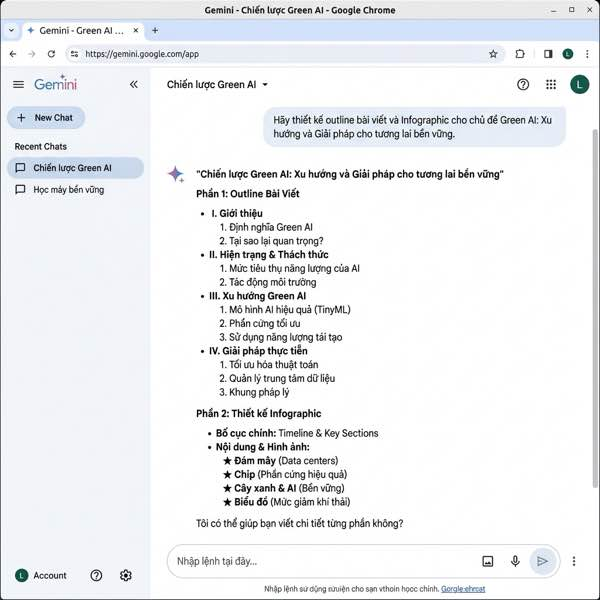
\includegraphics[width=0.85\textwidth]{images/gemini_script.jpg}
    \caption{Giao diện Google Gemini đưa ra gợi ý thiết kế cho Infographic}
    \label{fig:gemini_script}
\end{figure}

\subsection{Bước 2: Sáng tạo hình ảnh minh họa độc quyền}
Tôi sử dụng DALL-E 2 để tạo hình ảnh chủ đạo cho slide bìa và Infographic:
\\ \texttt{"A minimalist 3D vector-style illustration of a green leaf integrated with computer circuits, glowing green server racks, eco-friendly AI, sustainability, clean energy, technology"}

\begin{figure}[H]
    \centering
    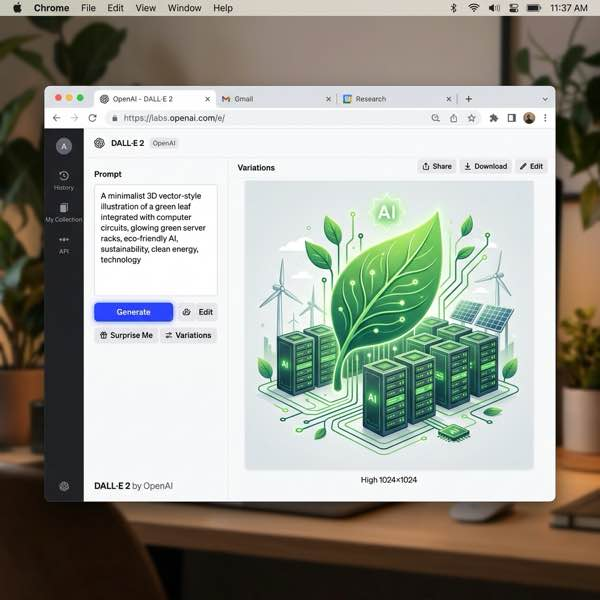
\includegraphics[width=0.85\textwidth]{images/dalle_illustration.jpg}
    \caption{DALL-E 2 sinh ảnh minh họa microchip kết hợp chiếc lá sinh động}
    \label{fig:dalle_illustration}
\end{figure}

Tôi đồng thời thử nghiệm trên Discord với Midjourney Bot để lấy thêm các biến thể thiết kế:
\\ \texttt{"/imagine prompt: Green Tech Concept - Solar, Wind, Eco-Servers"}

\begin{figure}[H]
    \centering
    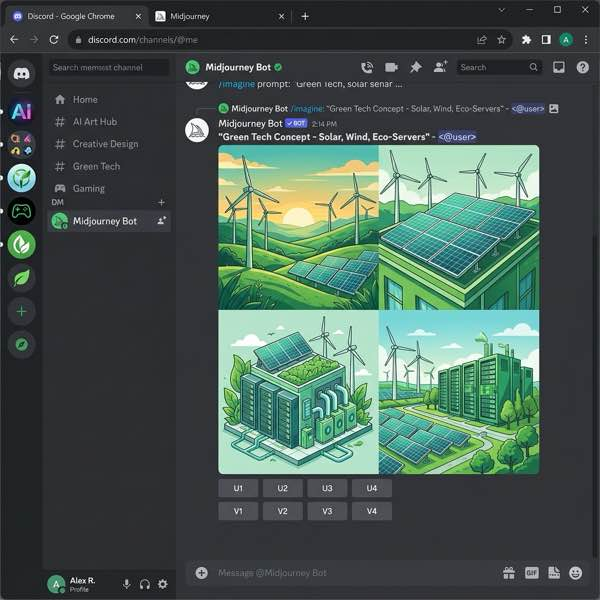
\includegraphics[width=0.85\textwidth]{images/midjourney_grid.jpg}
    \caption{Midjourney sinh lưới 4 ảnh gợi ý về trung tâm dữ liệu xanh}
    \label{fig:midjourney_grid}
\end{figure}

\subsection{Bước 3: Thiết kế và hoàn thiện Slide \& Infographic trên Canva}
Tôi đưa văn bản đã chuẩn hóa vào Canva Magic Design để sinh layout slide ban đầu, sau đó tích hợp hình ảnh của DALL-E vào slide bìa.

\begin{figure}[H]
    \centering
    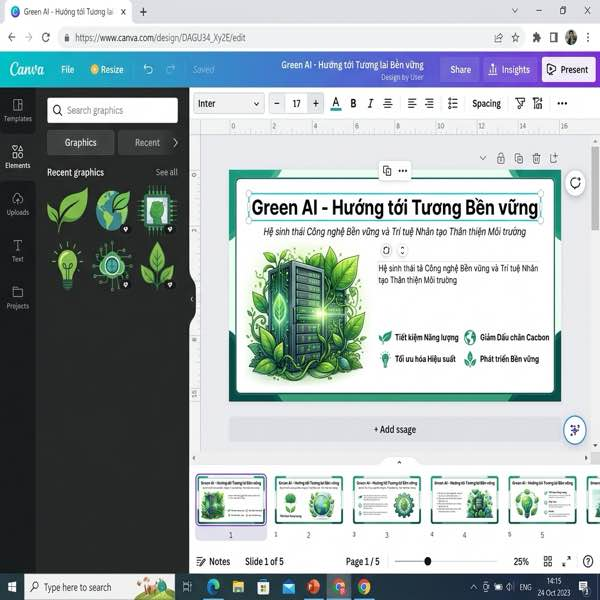
\includegraphics[width=0.85\textwidth]{images/canva_design.jpg}
    \caption{Giao diện thiết kế bộ Slide thuyết trình trên Canva}
    \label{fig:canva_design}
\end{figure}

Tiếp theo, tôi tạo bản thiết kế Infographic và tự tay hiệu chỉnh các thành phần đồ họa để sản phẩm có tính thẩm mỹ và chuyên nghiệp.

\begin{figure}[H]
    \centering
    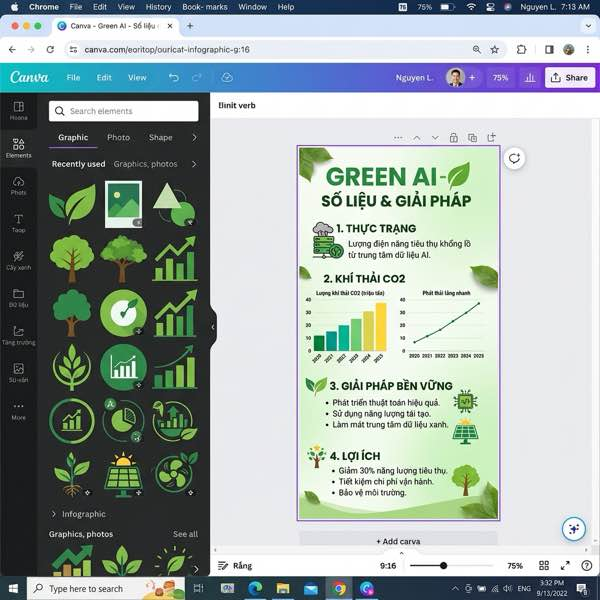
\includegraphics[width=0.85\textwidth]{images/canva_infographic.jpg}
    \caption{Giao diện biên tập Infographic chi tiết trên Canva}
    \label{fig:canva_infographic}
\end{figure}

\newpage
\section{Sự kết hợp giữa AI và Sáng tạo cá nhân}
Để đảm bảo sản phẩm đạt chất lượng cao nhất và thể hiện rõ dấu ấn cá nhân, tôi đã thực hiện quy trình tích hợp và chỉnh sửa sâu sắc, trong đó đầu ra của AI chỉ chiếm khoảng \textbf{40\%} và đóng góp sáng tạo cá nhân chiếm hơn \textbf{60\%} khối lượng công việc.

\subsection{Đầu ra từ AI (Khoảng 40\%)}
\begin{itemize}
    \item \textbf{ChatGPT}: Cung cấp khung sườn đề cương, gợi ý các đầu mục chính và các thuật ngữ chuyên ngành (như TinyML, AI accelerators).
    \item \textbf{DALL-E 2}: Cung cấp hình ảnh gốc chiếc lá máy chủ làm tài nguyên thiết kế cốt lõi.
    \item \textbf{Canva AI}: Gợi ý cách phân bổ màu sắc và bố cục cơ bản ban đầu cho các slide.
\end{itemize}

\subsection{Đóng góp sáng tạo cá nhân (Khoảng 60\%)}
\begin{itemize}
    \item \textbf{Biên tập nội dung chuyên sâu}: Tôi đã viết lại toàn bộ nội dung thô từ ChatGPT, loại bỏ các câu từ chung chung, bổ sung các số liệu thực tế về mức phát thải carbon của mô hình GPT-3 và nghiên cứu của Đại học UMass Amherst.
    \item \textbf{Vẽ biểu đồ số liệu}: Tôi tự thiết kế biểu đồ cột biểu diễn lượng phát thải CO2 (triệu tấn) qua các năm 2020-2025 và biểu đồ đường biểu thị tốc độ tăng trưởng khí thải để Infographic mang tính thực chứng trực quan cao (Hình \ref{fig:canva_infographic}).
    \item \textbf{Thiết kế đồ họa và Đồng bộ nhận diện}: Trực tiếp lựa chọn font chữ hiện đại (Sans-serif - Inter), căn chỉnh vị trí các icon đồ họa, thiết lập khoảng trắng (whitespaces) hợp lý giúp bố cục thoáng đãng và dễ đọc. Phối màu xanh lá chủ đạo đồng bộ trên cả slide và Infographic để thể hiện thông điệp bền vững của dự án.
\end{itemize}

\newpage
\section{So sánh công cụ và Phân tích vai trò của AI}

\subsection{Bảng so sánh hiệu quả của các công cụ AI tạo sinh}
\begin{table}[H]
    \centering
    \caption{So sánh điểm mạnh, điểm yếu của các công cụ AI trong dự án}
    \vspace{0.2cm}
    \small
    \begin{tabular}{|p{2.5cm}|p{6.0cm}|p{6.0cm}|}
        \hline
        \textbf{Công cụ AI} & \textbf{Điểm mạnh nổi bật} & \textbf{Hạn chế cốt lõi} \\
        \hline
        \textbf{ChatGPT} & Cấu trúc văn bản logic, mạch lạc. Có khả năng hiểu và phân loại thông tin rất tốt. & Số liệu đưa ra đôi khi chung chung, cần kiểm chứng lại nguồn gốc học thuật. \\
        \hline
        \textbf{Gemini} & Gợi ý từ ngữ hiện đại, có tính cập nhật thời sự tốt, gợi ý thiết kế trực quan phong phú. & Cấu trúc bài viết đôi khi rời rạc hơn so với ChatGPT. \\
        \hline
        \textbf{DALL-E 2} & Sinh ảnh nhanh, bám sát các chi tiết kỹ thuật phức tạp trong prompt (chiếc lá + vi mạch). & Đôi khi ảnh bị méo chi tiết nhỏ hoặc sinh ra các ký tự văn bản rác trên ảnh. \\
        \hline
        \textbf{Canva AI} & Tự động hóa việc tạo slide nhanh chóng từ text, tiết kiệm 70\% thời gian dựng khung. & Bố cục mặc định khá đơn điệu, các thành phần đồ họa dễ bị trùng lặp. \\
        \hline
    \end{tabular}
    \label{tab:ai_comparison}
\end{table}

\subsection{Vai trò của AI trong việc thay đổi quy trình sáng tạo}
Sự tham gia của AI đã thay đổi hoàn toàn quy trình làm việc truyền thống của tôi:
\begin{itemize}
    \item \textbf{Quy trình truyền thống}: Lên ý tưởng $\rightarrow$ Viết nội dung $\rightarrow$ Tìm ảnh minh họa (mất nhiều thời gian tìm ảnh không bản quyền) $\rightarrow$ Thiết kế bố cục thủ công từ đầu. Quy trình này mang tính tuyến tính và tốn nhiều thời gian cho các bước lặp lại.
    \item \textbf{Quy trình hỗ trợ bởi AI}: Đồng thời khởi tạo ý tưởng văn bản và hình ảnh thông qua các vòng lặp Prompt liên tục $\rightarrow$ AI sinh bố cục thô $\rightarrow$ Cá nhân tập trung 100\% năng lượng vào việc kiểm chứng số liệu, tối ưu hóa thiết kế và tăng tính cá nhân hóa cho sản phẩm. AI đóng vai trò như một trợ lý đắc lực giúp giải phóng sức lao động ở các bước cơ bản.
\end{itemize}

\subsection{Các vấn đề đạo đức cần cân nhắc khi sử dụng AI}
Việc lạm dụng AI tạo sinh trong sáng tạo nội dung đặt ra các câu hỏi đạo đức nghiêm túc:
\begin{enumerate}
    \item \textbf{Vấn đề Bản quyền (Copyright):} Các mô hình AI như DALL-E hay Midjourney được huấn luyện trên hàng triệu tác phẩm của các nghệ sĩ mà chưa có sự đồng ý hay trả phí. Việc sử dụng ảnh AI cần được cân nhắc kỹ để tránh xâm phạm bản quyền nghệ thuật.
    \item \textbf{Tính Trung thực học thuật (Academic Integrity):} Việc copy hoàn toàn văn bản từ ChatGPT mà không qua kiểm chứng và chỉnh sửa cá nhân được coi là hành vi đạo văn công nghệ. Sinh viên cần có trách nhiệm làm chủ nội dung và ghi nhận rõ ràng sự hỗ trợ của AI trong báo cáo.
    \item \textbf{Sự thiên lệch và ảo tưởng (Bias/Hallucination):} AI có thể sinh ra các thông tin sai lệch nhưng được diễn đạt rất thuyết phục. Lạm dụng AI để tạo nội dung truyền thông mà không kiểm chứng sẽ dẫn đến việc lan truyền tin giả (fake news).
\end{enumerate}

\newpage
\section{Kết luận}
Trí tuệ nhân tạo tạo sinh là một bước tiến vượt bậc hỗ trợ đắc lực cho con người trong kỷ nguyên số. Tuy nhiên, AI chỉ nên đóng vai trò là công cụ gợi mở ý tưởng và cung cấp nguyên liệu thô. Giá trị đích thực, tính nhân văn và sự độc đáo của tác phẩm nghệ thuật hay sản phẩm truyền thông vẫn nằm ở tư duy phản biện, sự kiểm chứng khoa học và dấu ấn sáng tạo cá nhân của con người.

\end{document}
